\section{Pebbling Game and Space}
\label{sec:pebbling-game}

%Todo: Discuss relation to resolution space complexity further
Pebbling games denote a family of games played on graphs where nodes are marked and unmarked throughout the rounds of the games.
The goal of these games is to mark some designated node.
On top of how many rounds have to be played to achieve the goal, an interesting characteristic of a particular instance of a pebbling game is the maximal amount of nodes that are marked simultaneously in all rounds.
The latter characteristic is the one we are interested in, because it models space requirements, if marking a node is interpreted as having it in memory.
In the context of pebbling games it is common to use the phrase to (un)pebble a node for (un)marking it.
Pebbling games were introduced in the 1970's to model programming language expressiveness \cite{Pippenger1980,Walker1973} and compiler construction \cite{Sethi1975}. 
More recently, pebbling games have been used to investigate various questions in parallel complexity \cite{Chan2013} and proof complexity \cite{Ben-Sasson2009,Esteban2001,Nordstroem2009}. 
They are used to obtain bounds for space and time requirements and trade-offs between the two measures \cite{EmdeBoas1979,Ben-Sasson2002}.
Space requirements are modeled by the number of pebbles used. 
Time requirements are reflected by the number of rounds played.

\begin{definition}[Bounded Pebbling Game]
\label{def:pebbling-game}
The \emph{Bounded Pebbling Game} is played by one player on a DAG $G = (V,E)$ with one distinguished node $s \in V$.
The goal of the game is to pebble $s$, respecting the following rules:
\begin{enumerate}
	\item \label{rule:premises} A node $\n$ is pebbleable if and only if all predecessors of $\n$ in $G$ are pebbled and $\n$ is currently not pebbled.
	\item \label{rule:unpebbling} Pebbled nodes can be unpebbled in any round.
	\item \label{rule:onlyonce} Once a node has been unpebbled, it may not be pebbled in a later round.
\end{enumerate}
%Only pebbled nodes can be unpebbled and only unpebbled nodes can be pebbled.
The game is played in rounds.
Every round the player chooses a node $v \in V$, such that $v$ is pebbled or pebbleable.
The \emph{move} of the player in this round is $p(v)$, if $v$ is pebbleable and $u(v)$ if $v$ is pebbled, where $p(.)$ and $u(.)$ correspond to pebbling and unpebbling a node respectively.

\end{definition}

Note that due to rule \ref{rule:premises} the move in each round is uniquely defined by the chosen node $v$.
The distinction of the two kinds of moves is just made for presentation purposes.
Also note that as a consequence of rule \ref{rule:premises}, pebbles can be put on nodes without predecessors at any time.
When playing the Bounded Pebbling Game on a proof $\varphi$, the designated target node is its root.

In this work we investigate space requirements when time requirements are fixed.
Fixing time is a design choice and it corresponds to rule \ref{rule:onlyonce}.
Including this rules sets a bound $O(|V|)$ for the number of rounds played and the number of pebbling moves is exactly $|V|$, since every node has to be pebbled exactly once.

\begin{definition}[Strategy]
\label{def:strategy}
A \emph{pebbling strategy} $\sigma$ for the Bounded Pebbling Game, played on a DAG $G = (V,E)$ and distinguished node $s$, is a sequence of moves $(\sigma_1,\ldots,\sigma_n)$ of the player such that $\sigma_n = p(s)$.
\end{definition}

The following definition allows to measure how many pebbles are required to play the Bounded Pebbling Game on a given graph.

\begin{definition}[Pebbling number]
The \emph{pebbling number of a pebbling strategy} $(\sigma_1,\ldots,\sigma_n)$ is 
$ max_{\indexIn{i}{1}{n}}|\{ \n \in V \mid \n \text{ is pebbled in round } i\}| $.
The \emph{pebbling number of a DAG $G$ and node $s$} is the minimum pebbling number of all pebbling strategies for $G$ and $s$.
\end{definition}

Note that Definitions \ref{def:pebbling-game} and \ref{def:strategy} leave the player freedom when to do unpebbling moves.
With the aim of finding strategies with low pebbling numbers, for every unpebbling move there is a canonical round make them, as shown below.

The Bounded Pebbling Game from Definition \ref{def:pebbling-game} differs from the Black Pebbling Game discussed in \cite{Hertel2007,Pippenger1982} in two aspects. 
Firstly, the Black Pebbling Game does not include rule \ref{rule:onlyonce}. 
Excluding this rule allows for pebbling strategies with lower pebbling numbers (\cite{Sethi1975} has an example on page 1), at the expense of an exponential upper bound on the number of rounds \cite{EmdeBoas1979}.
Secondly, when pebbling a node in the Black Pebbling Game, one of its predecessors' pebbles can be used instead of a fresh pebble (i.e. a pebble can be moved). 
The trade-off between moving pebbles and using fresh ones is discussed in \cite{EmdeBoas1979}. 
Deciding whether the pebbling number of a graph $G$ and node $s$ is smaller than $k$ is PSPACE-complete in the absence of rule \ref{rule:onlyonce} \cite{Gilbert1980} and NP-complete when rule \ref{rule:onlyonce} is included \cite{Sethi1975}.

Our view of the game is such that every round of the game corresponds to an I/O operation and, if the action of the player is to pebble a node, the processing of the node.
The goal of proof compression is to make proof processing less expensive, therefore admitting exponentially many I/O operations and processing steps in the worst case is not a viable option.
That is the reason why we chose the Bounded Pebbling Game for our purpose.
In the Bounded Pebbling Game the number of rounds is linear in the number of nodes.

In order to process a node according to Definition \ref{def:proof-processing}, the results of processing its premises are used and therefore have to be stored in memory.
The requirement of having premises in memory corresponds to rule \ref{rule:premises} of the Bounded Pebbling Game. 
A node that has been processed can be removed from memory, which corresponds to rule \ref{rule:unpebbling}.
Note that removing a node and its results too early in combination with \ref{rule:onlyonce} makes it impossible to process the whole proof.
The optimal moment to remove a node from memory is uniquely determined by the order nodes are processed (see Theorem \ref{theorem:canonical}).

Definition \ref{def:proof-processing} does not specify in which order to process nodes.
The order in which nodes are processed is essential for the memory consumption, just like the order of pebbling nodes in the pebbling game is essential for the pebbling number.
The following definition allows us to relate pebbling strategies with orderings of nodes.

\begin{definition}[Topological Order]
\label{def:topological-order}
A topological order of a proof $\varphi$ with nodes $V$ is a total order relation $\prec$ on $V$, such that 
$\text{for all } \n \in V \text{, for all } p \in \Premises{\n}{\varphi}:
p \prec v$.
A sequence of moves $(\sigma_1,\ldots,\sigma_n)$ in the pebbling game \emph{respects} a topological order $\prec$ if for all $j,i \in \{1,\ldots,n\}$ such that $\sigma_j = p(v_j)$ and $\sigma_i = p(v_i)$ it is true that $j < i$ if and only if $\n_j \prec \n_i$.
\end{definition}

A topological order $\prec$ of a proof $\varphi$ can be represented as a sequence $(v_1,\dots,v_n)$ of proof nodes, by defining $\prec \defeq \{(v_i,v_j) \mid 1 \leq i < j \leq n\}$. 
The requirement that topological orders premises lower than their children corresponds to rule \ref{rule:premises} of the Bounded Pebbling Game.
The antisymmetry together with the fact that $V = \{v_1,\dots,v_n\}$ correspond to rule \ref{rule:onlyonce}.
Theorem \ref{theorem:canonical} shows that the moments for unpebbling moves are predefined by the pebbling moves, when the goal is to find strategies with small pebbling numbers.
Therefore there is a bijection between topological orders and canonical pebbling strategies.

\begin{definition}[Canonical Topological Pebbling Strategy]
\label{def:canonstrat}
The \emph{canonical topological pebbling strategy} $\sigma$ for a proof $\varphi$, its root node $s$ and a topological order $\prec$ represented as a sequence $(v_1,\dots,v_n)$ is defined recursively:
$$
\begin{array}{l}
\sigma_1 = p(v_1) \\
\sigma_i = 
	\left\{
	\begin{array}{ll}
		%u(v) & \text{ if for all } c \in \Children{v}{\varphi}: \\
		       %& \quad \text{ there exists }k < i, \sigma_k = p(u) \text{ and }\\
					 %& \quad \text{ for all } l: k < l < i, \sigma_l \neq u(v) \\
		%u(v) & \text{ for all } c \in \Children{v}{\varphi} \text{ exists } k < i, \sigma_k = p(u) \text{ and for all }l: k < l < i, \sigma_l \neq u(v) \\
		u(v) & \text{if for all } c \in \Children{v}{\varphi} \text{ exists } k < i \text { such that } \sigma_k = p(c)\\
		p(v) & \text{otherwise, where } v = min_{\prec}(w \mid \text{ for all } l < i: \sigma_l \neq p(w))
	\end{array}
	\right.
	%finished(v,i) := \text{ for all} c \in \Children{v}{\varphi} \text{ exists } k < i, \sigma_k = p(u) \text{ and for all } k < l < i, \sigma_l \neq u(v) 
\end{array}
$$
\end{definition}

The following theorem shows that unpebbling moves can be omitted from strategies for the Bounded Pebbling Game, when the goal is to produce strategies with low pebbling numbers.

\begin{theorem}
\label{theorem:canonical}
The canonical pebbling strategy has the minimum pebbling number among all pebbling strategies that respect the topological order $\prec$.
\end{theorem}
\begin{proof}
%Let $\sigma = (\sigma_1,\ldots,\sigma_n)$ be the canonical pebbling strategy for $\prec$ and let $\sigma' = (\sigma'_1,\ldots,\sigma'_n)$ be a pebbling strategy respecting $\prec$ such that $\sigma \neq \sigma'$.
%All the pebbling strategies respecting $\prec$ differ only in the order of unpebbling moves.
Definition \ref{def:canonstrat} prioritizes unpebbling over pebbling moves.
Therefore the canonical topological pebbling strategy makes unpebbling moves as soon as possible.
Consider the moment for unpebbling an arbitrary node $v$ in the canonical pebbling strategy. 
Unpebbling it later could only possibly increase the pebble number. 
To reduce the pebble number, $v$ would have to be unpebbled earlier than some preceding pebbling move. 
But, by definition of canonical pebbling strategy, the immediately preceding pebbling move pebbles the last child of $v$ w.r.t. $\prec$. 
Therefore, unpebbling $v$ earlier would make it impossible for its last child to be pebbled later without violating the rules of the game.
\end{proof}

As a consequence of Theorem \ref{theorem:canonical} finding pebbling strategies with low pebbling numbers can be reduced to constructing topological orders.
The memory required to process a proof using some topological order can be measured by the pebbling number of the canonical pebbling strategy corresponding to the order.
We are now ready to define another measure on proofs, which we call space.

\begin{definition}[Space of a Proof]
\label{def:space measure}
The \emph{space} $\pspace{\varphi}{\prec}$ 
of a proof $\varphi$ and a topological order $\prec$ is the pebbling number of the canonical topological pebbling strategy of $\varphi$, its root and $\prec$.
\end{definition}

\begin{example}

Consider the proof displayed in Figure \ref{fig:spaceproof}.
The indices below the proof nodes indicate a topological order that has pebbling number four.
The implicit unpebbling moves are to unpebble node $1$ after pebbling node $3$, as well as unpebbling nodes $2$ and $4$ after pebbling node $5$.
Before unpebbling nodes $2$ and $4$, nodes $2,3,4,5$ are pebbled which is the maximal amount of pebbles placed on the graph at any time.
It is easy to see, that there is no topological order that has a canonical pebbling strategy with a lower pebbling number.

%\begin{figure}[!h]
%
\centering
\begin{tikzpicture}[node distance=2.5cm]
	
	\proofnode[align=center,font=\small]{root}{$\bot$\\$6$};
	\proofnode[above left of=root,align=center,font=\small]{n3}{$a$\\$3$};
	\proofnode[above right of=root,align=center,font=\small]{n5}{$\neg a$\\$5$};
	\proofnode[above left of=n3,align=center,font=\small]{n1}{$a,\neg b$\\$1$};
	\proofnode[above right of=n3,align=center,font=\small]{n2}{$b$\\$2$};
	\proofnode[above right of=n5,align=center,font=\small]{n4}{$\neg a, \neg b$\\$4$};
	\drawchildren{n5}{n2}{n4};
	\drawchildren{root}{n3}{n5};
	\drawchildren{n3}{n1}{n2};
	
\end{tikzpicture}


%\caption{A Simple Proof}
%\label{fig:spaceproof}
%\end{figure}

\end{example}

The problem of compressing the space of a proof $\varphi$ and a topological order $\prec$ is the problem of finding another topological order $\prec'$ such that $\pspace{\varphi}{\prec'} < \pspace{\varphi}{\prec}$. The following theorem shows that the number of possible topological orders is very large and hence, enumeration is not a feasible option when trying to find a good topological order.

\begin{theorem}
\label{theorem:enumeration}
There is a sequence of proofs $(\varphi_1,\ldots,\varphi_m,\ldots)$ such that $\plength{\varphi_m} \in O(m)$ and $|T(\varphi_m)| \in \Omega(m!)$, where $T(\varphi_m)$ is the set of possible topological orders for $\varphi_m$.
\end{theorem}
\begin{proof}
Let $\varphi_m$ be a perfect binary tree with $m$ axioms. Clearly, $\plength{\varphi_m} = 2m-1$.
Let $(\n_1,\ldots,\n_n)$ be a topological order for $\varphi_m$. 
Let $\Axioms{\varphi} = \{\n_{k_1},\ldots,\n_{k_m}\}$, then\\ $(\n_{k_1},\ldots,\n_{k_m},\n_{l_1},\ldots,\n_{l_{n-m}})$, where $(l_1,\ldots,l_{n-m}) = (1,\ldots,n) \setminus (k_1,\ldots,k_m)$, is a topological order as well. 
Likewise, $(\n_{\pi({k_1})},\ldots,\n_{\pi({k_m})},\n_{l_1},\ldots,\n_{l_{n-m}})$ is a topological order, for every permutation $\pi$ of $\{k_1,\ldots,k_m\}$. There are $m!$ such permutations, so the overall number of topological orders is at least factorial in $m$ (and also in $n$).
\end{proof}

